% \section{Appendix}
% \parttoc % Insert the appendix TOC

% \subsection{KG-specialized LLM Fine-tuning}\label{app:finetuning}
% To enhance the ability of LLMs and make them specialized for KG reasoning, we fine-tune lightweight LLMs on the graph-constrained decoding task. Specifically, given a question $q$, the models are optimized to generate relevant reasoning paths $\vw_\vz$ that are helpful for answering the question, then provide a hypothesis answer $a$ based on it. The training objective can be formulated as:
% \begin{equation}
%     \max_{\theta} \mathbb{E}_{(q, \vw_\vz, a) \sim \mathcal{D}} \log P_\theta(a, \vw_\vz | q) = 
% \end{equation}


\RE{
\section{Detailed Related Work on KG-enhanced LLMs}\label{app:related_work}
Knowledge graph (KG), as a structured representation of factual knowledge, has been widely used to enhance the factual knowledge and reasoning abilities of LLMs \citep{pan2023unifying,liang2024simple} by reducing the hallucinations \citep{nguyen-etal-2024-direct,dhuliawala2024chain,lv2024coarsetofine}.
%
In this section, we provide a detailed review of the related work on KG-enhanced LLMs, which can be categorized into two paradigms: retrieval-based and agent-based methods.

\noindent\textbf{Retrieval-based Methods.} Retrieval-based methods retrieve relevant facts from KGs with an external retriever and then feed them into the inputs of LLMs for reasoning. These methods aim to provide LLMs with external knowledge to enhance their reasoning abilities \citep{li2025g}. For example, KD-CoT \citep{wang2023knowledge} retrieves relevant knowledge from KGs to generate faithful reasoning plans for LLMs. EWEK-QA \citep{dehghan-etal-2024-ewek} enriches the retrieved knowledge by searching from both KGs and the web. RoG \citep{luo2024rog} proposes a planning-retrieval-reasoning framework that retrieves reasoning paths from KGs to guide LLMs conducting faithful reasoning. GNN-RAG \citep{mavromatis2024gnn} adopts a lightweight graph neural network to effectively retrieve from KGs. GNN-RAG+RA \citep{mavromatis2024gnn} combines the retrieval results of both RoG and GNN-RAG to enhance the reasoning performance. GFM-RAG \citep{luo2025gfmrag} utilizes KG as the structural index of knowledge and designs a graph foundation model to reason on KGs and retrieve relevant knowledge for LLMs. Studies have also been proposed to retrieve from dynamic KGs to enhance the temporal reasoning abilities of LLMs \citep{wang2024large,liang2023learn}. However, these methods may suffer from the retrieval accuracy, which limits the reasoning performance. 

\noindent\textbf{Agent-based Methods.} Agent-based methods treat LLMs as agents that iteratively interact with KGs to find reasoning paths and answers. For example, StructGPT \citep{jiang2023structgpt} treats LLMs as agents to interact with KGs to find a reasoning path leading to the correct answer. ToG \citep{sunthink} extends the method and conducts reasoning on KGs by exploring multiple paths and concludes the final answer by aggregating the evidence from them. EffiQA \citep{jiang2024kg} proposes an efficient agent-based method to reason on KGs. Plan-on-Graph \citep{chenplan} proposes an adaptive planing paradigm to decompose the question into sub-tasks and guide the LLMs to reason on KGs. Debate on Graph \citep{ma2024debate} asks LLM as agents to debate with each other to gradually simplify complex questions and find the correct answers. SymAgent \citep{liu2025symagent} introduces a collaborative agent framework that autonomously utilizes tools to integrate information from KGs and external documents, tackling the problem of KG incompleteness. 
Although these methods are effective, they face high computational costs and challenges in designing the interaction process.

}

\RE{
    \section{KG-Trie Construction}\label{app:kg_trie}
    KG-Trie converts KG structures into the format that LLMs can handle. It can been incorporated into the LLM decoding process as constraints, allowing for faithful reasoning paths that align with the graph’s structure.
    %
    The KG-Trie can be either pre-computed for fast inference or constructed on-demand to minimize pre-processing time.

    \subsection{Construction Strategies}
    \noindent\textbf{Offline Construction.} The KG-Trie can be pre-computed offline, allowing them to be used during inference at no additional cost. Instead of constructing the KG-Trie for all entities in the KG, we could only construct the KG-Trie for certain entities. We can select the entities based on their popularity, importance, or the frequency of their occurrence in the questions.

    \noindent\textbf{On-demand Construction.} Alternatively, we can construct the KG-Trie on-demand. When a question is given, we first identify the question entities with named entity recognition (NER) tools. Then, we retrieve the question-related subgraphs around the question entities from the KGs. Finally, we construct a question-specific KG-Trie based on the retrieved subgraphs. The KG-Trie is then used to guide the LLMs to reason on the KGs.

    \noindent\textbf{Dynamic Cache for KG-Trie Construction.} Users can also develop their own strategies to balance pre-processing and inference overhead. For example, we can maintain a dynamic cache to store the KG-Trie for the most frequently asked questions, as shown in \Cref{fig:cache}. When a new question is given, they first check whether the KG-Trie for the question is in the cache. If it is, they directly use the KG-Trie for inference. Otherwise, they construct a question-specific KG-Trie on-demand. The cache can be updated periodically to remove the least frequently used KG-Trie and add the new ones.

    \begin{figure}[htb]
    \begin{center}
        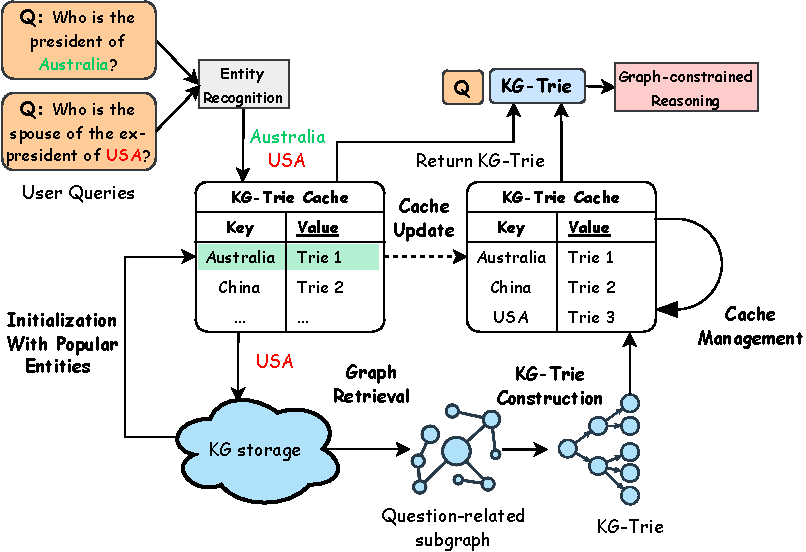
\includegraphics[width=.8\columnwidth]{images/kg-trie-cache.pdf}
      \end{center}
    %   \vspace{-14pt}
      \caption{The illustration of dynamic cache for KG-Trie construction.}
    %   \vspace{-16pt}
    \label{fig:cache}
  \end{figure}

    \subsection{Time and Space Complexity Analysis}
    The time and space complexity for KG-Trie construction is affordable and can be easily improved in industry-level applications to support billions of scale graphs. To support this, we provide detailed theoretical analysis and empirical evidence. In experiments, we adopt the breadth-first search, whose complexities are:

    \subsubsection{Theoretical Analysis}
    \noindent\textbf{Time Complexity.}  Constructing the KG-Trie involves a BFS traversal to explore paths up to a maximum length of $L$ starting from certain entities. The time complexity of this traversal is $O(E^{L})$, where $E$ is the average number of edges per entity, and $L$ is the maximum path length. BFS ensures that all reachable paths up to length $L$ are considered. However, BFS can be replaced with other efficient graph-traversing algorithms, such as random walk \citep{xia2019random} to further improve efficiency.

    \noindent\textbf{Space Complexity.} The space complexity of the KG-Trie depends on the number of unique paths and their tokenized representations. In the worst case, the space complexity is $O(E^L \times T)$, where $T$ represents the average number of tokens per path. Trie structures are efficient for storing shared prefixes, which reduces redundancy and optimizes memory usage. Moreover, it supports efficient traversal of reasoning paths in constant time.

    \subsubsection{Empirical Analysis}
    We have provided the average BFS running time and space consumption of the KG-Trie construction to demonstrate its efficiency. The system settings are illustrated at \Cref{tab:system_settings}.

    \begin{table}[h!]
        \centering
        \caption{System settings overview for efficiency experiments.}\label{tab:system_settings}
        \begin{tabular}{@{}l|l@{}}
            \toprule
            System Setting     & Specification                               \\
            \midrule
            CPU                & Intel(R) Xeon(R) Silver 4214R CPU @ 2.40GHz \\
            \midrule
            Memory             & 32G                                         \\
            \midrule
            BFS Implementation & Virtuoso SPARQL                                    \\
            \midrule
            Space Storage      & Pickle                                      \\
            \bottomrule
        \end{tabular}
    \end{table}

    In the experiment, we build the KG-Trie for all question entities of WebQSP dataset and measure the average running time and space consumption. The BFS is executed on the Freebase KG stored in a Virtuoso database \citep{erling2009rdf}. We retrieve the $L$-hop paths, then save the constructed KG-Trie with Pickle. The statistics show that both running time and space usage are acceptable when $L<=3$, which highlights efficiency in KG-Trie construction. 
    %
    Although a larger hop can lead to better coverage of the possible answer, it would significantly increase the time and space complexity. Thus, we set hops to 2 or 3 in experiments to balance between efficiency and effectiveness. Notably, time can be further reduced by utilizing multi-threading. Space consumption can be optimized by storing data in a database.


    \begin{table}[]
        \centering
        \caption{Average running time and space utilization of the KG-Trie construction.}\label{tab:time_and_sapce}
        % \resizebox{\textwidth}{!}{%
        \begin{tabular}{@{}ccc@{}}
            \toprule
            Hop & Avg. Running Time (s) & Space (Mb) \\ \midrule
            L=1 & 0.0058                & 0.4        \\
            L=2 & 0.0133                & 0.5        \\
            L=3 & 0.0219               & 2.5        \\\bottomrule
        \end{tabular}%
        % }
    \end{table}

    \subsubsection{Time Consumption Breakdown}
    In addition, we have provided a detailed breakdown of the time consumption for each component involved in the KG-Trie construction. As shown in \Cref{tab:breakdown}, the overall time for constructing the KG-Trie under the open-end setting is approximately 0.28 seconds. This includes the time for all necessary stages, such as Named Entity Recognition, Entity Linking, graph retrieval, tokenization, and trie construction.

    \begin{table}[]
        \centering
        \caption{Breakdown of the time consumption for each component involved in the KG-Trie construction.}
        \label{tab:breakdown}
        \resizebox{\textwidth}{!}{%
        \begin{tabular}{@{}llll@{}}
        \toprule
        Component                      & Description                                                            & Implementation                                   & Time (s) \\ \midrule
        Named Entity Recognition (NER) & Identify mentioned entities in user questions                          & Spacy                                            & 0.0059   \\
        Entity Linking (NL)            & Link to entities in KGs                                                & ColBERTv2                                        & 0.0457   \\
        Graph Retrieval                & Retrieve question-relevant subgraphs for KG-Trie construction (Eq. 3). & 2-hop BFS implemented with SPARQL.               & 0.0133   \\
        Tokenizer                      & Tokenize paths into tokens for building LLM constraints (Eq. 4).       & Llama-3-8B Tokenizer implemented by Huggingface. & 0.1227   \\
        Trie construction              & Store the tokenized paths with Trie (Eq. 5).                           & Python MARISA Trie                               & 0.0962   \\\midrule
        \textbf{Total}                          &                                                                        &                                                  & \textbf{0.2838}   \\ \bottomrule
        \end{tabular}%
        }
        \end{table}

    \subsection{Strategies for Optimizing Efficiency}
    We provide several strategies that can be used to further speed up the KG-Trie construction.

    \noindent\textbf{Parallel Processing:} As the KG-Trie is independently constructed for each entity, it can be easily scaled with parallel processing. We provide the total running time of constructing 2-hop KG-Trie of all question entities in WebQSP dataset in \Cref{tab:multi-processing} to show the improvement of parallel processing. It shows that the efficiency can be greatly improved with parallel processing. This parallel nature enables it to be executed on distributed computing systems such as Hadoop and Spark in real-world applications.

    \begin{table}[h!]
        \centering
        \caption{Total running time and improvement under different processing threads.}
        \label{tab:multi-processing}
        % \resizebox{\textwidth}{!}{%
        \begin{tabular}{@{}ccc@{}}
            \toprule
            Total time (s) & Total Time (min) & Improvement \\ \midrule
            Thread=1       & 4.03             & 100\%       \\
            Thread=4       & 3.21             & 126\%       \\
            Thread=10      & 2.31             & 174\%       \\
            Thread=20      & 1.92             & 210\%       \\ \bottomrule
        \end{tabular}%
        % }
    \end{table}

    \noindent\textbf{Efficiency Graph Traversal Algorithms:} The BFS or DFS enumerates all the paths around the entities which might lead to computational overhead. However, they can be easily replaced with other graph traversal algorithms, such as random walk, to reduce time complexity.

    % \noindent\textbf{On-demand KG-Trie Construction:} Instead of pre-computing the KG-Trie, the Trie can be constructed on-demand with new questions asked. In this case, we do not need to construct the KG-Trie for entities in KGs, which many of them are never used at all. Meanwhile, we can retrieve a question-related graph to reduce overhead in graph traversal.

    \noindent\textbf{Combination with Graph Retrieval Algorithms:} To reduce the overhead of graph traversal, we can construct the KG-Trie on the question-related subgraphs. To this end, our methods can be combined with other graph retrieval algorithms, such as GNN-RAG \citep{mavromatis2024gnn} and RoG \citep{luo2024rog}. They would retrieve meaningful and relevant paths from KGs to speed up the KG-Trie construction. However, the performance might be limited by the retrieval accuracy.

    \noindent\textbf{Reduce Entities Number:} Instead of constructing the KG-Trie for all entities in the KG, we could only construct the KG-Trie for certain entities. We can select the entities based on their popularity, importance, or the frequency of their occurrence in the questions.

    \subsection{Real-World Applicability}
    To support real-world applications with billion-scale KGs, KG-Trie construction can be implemented in industrial-level settings. For instance, billion-scale KGs can be stored in scalable graph databases like Neo4j. The parallel nature of KG-Trie construction allows it to be executed on distributed computing systems such as Hadoop and Spark, enabling pre-computation and offline storage. The constructed KG-Trie can then be stored in a database and loaded for inference without additional computation, facilitating real-time responses. To reduce the overhead in pre-processing, we can design a cache mechanism that only builds KG-Trie for popular accessed entities and caches them for faster inference. The illustration of the framework can be found in \Cref{fig:cache}.
}
\section{Datasets}\label{app:datasets}

\noindent\textbf{KGQA Datasets.} To compare the reasoning performance with existing methods, we use two benchmark KGQA datasets in this study: WebQuestionSP (WebQSP) \citep{yih2016value} and Complex WebQuestions (CWQ) \citep{talmor2018web}. To ensure fairness, we adopt the same train and test splits as previous works \citep{jiang2022unikgqa,luo2024rog}. Details of the datasets can be found in \Cref{tab:merged_stats}.

Both WebQSP and CWQ can be reasoned using Freebase KGs\footnote{\url{https://github.com/microsoft/FastRDFStore}} \citep{bollacker2008freebase}. To reduce the size of the KGs, we use a subgraph of Freebase by extracting all triples that start from question entities within the maximum reasoning hops provided by previous works\footnote{WebQSP: \url{https://huggingface.co/datasets/rmanluo/RoG-webqsp}, CWQ: \url{https://huggingface.co/datasets/rmanluo/RoG-cwq}} \citep{luo2024rog}. The statistics of the knowledge graphs are shown in \Cref{tab:kg}.

\noindent\textbf{Fine-tuning Datasets.} To enhance the KG reasoning ability of LLMs, we construct fine-tuning datasets by generating reasoning paths from the KGs. Specifically, we adopt the training split of WebQSP and CWQ, which contain 2,826 and 27,639 question-answer pairs, respectively. For each question, we find all the shortest reasoning paths on KGs that connect the question entity to the answer entity. We then convert the reasoning paths into formatted strings and pair them with the question-answer pairs with the template shown in \Cref{fig:path_gen_prompt}  to form the fine-tuning datasets. Since there could be multiple reasoning paths for a question, we generate multiple training instances paired with different reasoning paths for each question-answer pair. The fine-tuning datasets contain 28,307 and 181,602 question-reasoning path-answer triples for WebQSP and CWQ, respectively. The statistics of the fine-tuning datasets are shown in \Cref{tab:it-data}.

\noindent\textbf{Zero-shot Generalization Datasets.} To evaluate the transferability of \ourmethod, \RE{we further select three new KGQA datasets: FreebaseQA \citep{jiang2019freebaseqa}, CommonsenseQA (CSQA) \citep{talmor2019commonsenseqa} and MedQA-USMLE (MedQA) \citep{jin2021disease}}.\RE{FreebaseQA is an open-ended question answering dataset.} CSQA is a 5-way multiple choice QA dataset that involves reasoning with commonsense knowledge. MedQA is a 4-way multiple choice QA task that requires biomedical and clinical knowledge. \RE{FreebaseQA adopts the same Freebase KG used in WebQSP and CWQ.} For CSQA, we use the ConceptNet \citep{speer2017conceptnet}, which is a general-purpose KG that contains commonsense knowledge. For MedQA, we use a medical KG constructed from the Unified Medical Language System \citep{yasunaga2021qa}. The statistics of the knowledge graphs are shown in \Cref{tab:kg}. We respectively select 100 questions from each dataset. For each question, following previous studies \citep{feng2020scalable,yasunaga2021qa}, a 2-hop subgraph is extracted from the KGs to form the zero-shot generalization datasets.

% % \begin{wraptable}{r}{.35\columnwidth}
% \begin{table}[]
%     \centering
%     % \vspace{-3mm}
%     \caption{Statistics of datasets.}
%     \label{tab:dataset}
%     % \resizebox{.35\columnwidth}{!}{%
%     \begin{tabular}{@{}c|ccc@{}}
%         \toprule
%         Datasets & \#Train & \#Test & Max \#hop \\ \midrule
%         WebQSP   & 2,826   & 1,628  & 2         \\
%         CWQ      & 27,639  & 3,531  & 4         \\ \bottomrule
%     \end{tabular}%
%     % }
%     % \vspace{-3mm}
% % \end{wraptable} 
% \end{table}


% \begin{table}[]
%     \centering
%     \caption{Statistics of the number of answers for questions in WebQSP and CWQ.}
%     \label{tab:ans_dist}
%     %\resizebox{\textwidth}{!}{%
%     \begin{tabular}{@{}ccccc@{}}
%         \toprule
%         Dataset & \#Ans = 1 & 2 $\geq$ \#Ans $\leq$ 4 & 5 $\geq$ \#Ans $\leq$ 9 & \#Ans $\geq$ 10 \\ \midrule
%         WebQSP  & 51.2\%    & 27.4\%                  & 8.3\%                   & 12.1\%          \\
%         CWQ     & 70.6\%    & 19.4\%                  & 6\%                     & 4\%             \\ \bottomrule
%     \end{tabular}%

% \end{table}

% \begin{table}[]
%     \centering
%     \caption{Statistics of the question hops in WebQSP and CWQ.}
%     \label{tab:hop_dist}
%     %\resizebox{\textwidth}{!}{%
%     \begin{tabular}{@{}cccc@{}}
%         \toprule
%         Dataset & 1 hop                         & 2 hop   & $\geq$ 3 hop \\ \midrule
%         WebQSP  & 65.49                      \% & 34.51\% & 0.00\%       \\
%         CWQ     & 40.91                      \% & 38.34\% & 20.75\%      \\ \bottomrule
%     \end{tabular}%
%     %}
% \end{table}

% \begin{table}[]
%     \centering
%     \caption{Statistics of datasets, number of answers, and question hops.}
%     \label{tab:merged_stats}
%     \begin{tabular}{@{}c|ccc|cccc|c@{}}
%         \toprule
%         Dataset & \#Train & \#Test & Max \#hop & \#Ans = 1 & 2 $\geq$ \#Ans $\leq$ 4 & 5 $\geq$ \#Ans $\leq$ 9 & \#Ans $\geq$ 10 & 1 hop & 2 hop & $\geq$ 3 hop \\ \midrule
%         WebQSP  & 2,826   & 1,628  & 2         & 51.2\%    & 27.4\%                  & 8.3\%                   & 12.1\%          & 65.49\% & 34.51\% & 0.00\%       \\
%         CWQ     & 27,639  & 3,531  & 4         & 70.6\%    & 19.4\%                  & 6\%                     & 4\%             & 40.91\% & 38.34\% & 20.75\%      \\ \bottomrule
%     \end{tabular}%
% \end{table}

\begin{table}[h]
    \centering
    \caption{Statistics of datasets.}
    \label{tab:merged_stats}
    % \resizebox{\columnwidth}{!}{%
    \begin{tabular}{@{}c|cc|cccc@{}}
    \toprule
    \multirow{2}{*}{Dataset} & \multicolumn{2}{c|}{Dataset Statistics} & \multicolumn{4}{c}{Statistics of Answer Numbers}                                \\ \cmidrule(l){2-7} 
                             & \#Train             & \#Test            & \#Ans = 1 & 2 $\geq$ \#Ans $\leq$ 4 & 5 $\geq$ \#Ans $\leq$ 9 & \#Ans $\geq$ 10 \\ \midrule
    WebQSP                   & 2,826               & 1,628             & 51.2\%    & 27.4\%                  & 8.3\%                   & 12.1\%          \\
    CWQ                      & 27,639              & 3,531             & 70.6\%    & 19.4\%                  & 6\%                     & 4\%             \\ \bottomrule
    \end{tabular}%
    % }
\end{table}

\begin{table}[htb]
    \centering
    \caption{Statistics of fine-tuning datasets for graph-constrained decoding.}
    \label{tab:it-data}
    % \resizebox{\columnwidth}{!}{%
    \begin{tabular}{@{}ccc@{}}
        \toprule
        Total & WebQSP & CWQ \\ \midrule
        209,909     & 28,307                  & 181,602                \\ \bottomrule
    \end{tabular}%
    % }
\end{table}
\begin{table}[H]
    \centering
    \caption{Statistics of constructed knowledge graphs.}
    \label{tab:kg}
    %\resizebox{\textwidth}{!}{%
    \begin{tabular}{@{}cccc@{}}
        \toprule
        KG         & \#Entities & \#Relations & \#Triples \\\midrule
        Freebase   & 2,566,291
                   & 7,058      & 8,309,195               \\
        ConceptNet & 799,273    & 17           & 2,151,303   \\
        MedKG      & 9,958 & 15 & 49,974  \\

        \bottomrule
    \end{tabular}%
    %}
\end{table}

\section{Baselines}\label{app:baselines}
We compare \ourmethod with the 22 baselines grouped into three categories: 1) \emph{LLM reasoning methods}, 2) \emph{graph reasoning methods}, and 3) \emph{KG-enhanced LLM reasoning methods}. The details of each baseline are described as follows.

\noindent\textbf{LLM reasoning methods} only rely on LLMs for reasoning without utilizing external KGs. We include both the vanilla LLMs with different sizes and the LLMs with advanced reasoning mechanisms. Specifically, we consider the following baselines:
\begin{itemize}
    \item Qwen2-0.5B/1.5B.7B \citep{qwen2} provides a series of pre-trained LLMs with different sizes, including 0.5B, 1.5B, and 7B parameters.
    \item Llama-2-7B \citep{touvron2023llama} is a large-scale LLM pre-trained on a diverse range of tasks.
    \item Llama-3.1-8B \citep{llama3} is the updated version of Llama-2 with more powerful reasoning capabilities.
    \item ChatGPT \citep{chatgpt} is a powerful closed-source LLM that could follow instructions to conduct complex tasks.
    \item GPT-4o-mini \citep{gpt4o} is the new flagship model of OpenAI that could reason across different modalities and tasks.
    \item Few-shot prompt \citep{brown2020language} is a few-shot learning method that provides LLMs with a few examples in the prompts to conduct reasoning.
    \item CoT \citep{wei2022chain} is a chain-of-thought reasoning method that prompts LLMs to generate a chain of reasoning steps.
    \item Self-consistency \citep{wangself} generates multiple reasoning paths and selects the most consistent answer.
\end{itemize}

\noindent\textbf{Graph reasoning methods} focus on reasoning on KGs using graph neural networks (GNNs) \citep{wu2020comprehensive} or graph-based reasoning mechanisms. We include the following baselines:
\begin{itemize}
    \item GraftNet \citep{sun2018open} is a graph-based reasoning method that retrieves relevant subgraphs from KGs with entity linking.
    \item NSM \citep{he2021improving} utilizes the sequential model to mimic the multi-hop reasoning process on KGs.
    \item SR+NSM \citep{zhang2022subgraph} proposes a relation-path retrieval to retrieve subgraphs for multi-hop reasoning.
    \item ReaRev \citep{mavromatis2022rearev} is a GNN-based method that reasons on KGs by considering complex graph information.
    \item \RE{UniKGQA \citep{jiang2022unikgqa} is a unified framework that combines graph-based reasoning of GNNs and LLMs for KGQA.}
\end{itemize}

\noindent\textbf{KG-enhanced LLM reasoning methods} incorporate KGs to enhance the reasoning abilities of LLMs which can be further divided into retrieval-based and agent-based paradigms. We include the following baselines:

\emph{Retrieval-based methods} retrieve relevant facts from KGs with an external retriever and then feed them into the inputs of LLMs for reasoning:
\begin{itemize}
    \item KD-CoT \citep{wang2023knowledge} retrieves relevant knowledge from KGs to generate faithful reasoning plans for LLMs.
    \item EWEK-QA \citep{dehghan-etal-2024-ewek} enriches the retrieved knowledge by searching from both KGs and web.
    \item RoG \citep{luo2024rog} proposes a planning-retrieval-reasoning framework that retrieves reasoning paths from KGs to guide LLMs conducting faithful reasoning.
    \item GNN-RAG \citep{mavromatis2024gnn} adopts a lightweight graph neural network to effectively retrieve from KGs.
    \item GNN-RAG+RA \citep{mavromatis2024gnn} combines the retrieval results of both RoG and GNN-RAG to enhance the reasoning performance.
\end{itemize}

\emph{Agent-based methods} treat LLMs as agents that iteratively interact with KGs to find reasoning paths and answers:
\begin{itemize}
    \item ToG \citep{sunthink} conducts the reasoning on KGs by exploring multiple paths and concludes the final answer by aggregating the evidence from them.
    \item EffiQA \citep{jiang2024kg} proposes an efficient agent-based method to reason on KGs.
\end{itemize}

\section{Implementation Details and Experiment Settings}\label{app:implementation}
In this section, we will detail the implementation of \ourmethod as well as the experiment settings.

\noindent\textbf{Fine-tuning KG-specialized LLMs.} We fine-tune several lightweight LLMs ranging from 0.5B to 8B \citep{qwen2,touvron2023llama,llama3} on the fine-tuning datasets for 3 epochs. The batch size is set to 4 and the learning rate is set to 2e-5. We use the cosine learning rate scheduler policy with the warmup ratio set to 0.03. The training is conducted on 2 A100-80G GPUs for each model. The training time and memory usage are shown in \Cref{tab:training}.


\begin{table}[]
    \centering
    \caption{Training time and memory usage for different KG-specialized LLMs. }
    \label{tab:training}
    % \resizebox{\columnwidth}{!}{%
    \begin{tabular}{@{}lcc@{}}
    \toprule
    \multicolumn{1}{c}{Model} & Time   & Mem. Usage per GPU \\ \midrule
    Qwen2-0.5B                & 3.47h  & 10G            \\
    Qwen2-1.5B                & 4.11h  & 25G            \\
    Qwen2-7B                  & 14.37h & 81G            \\
    Llama-2-7B                & 13.93h & 80G            \\
    Llama-3.1-8B               & 14.52h & 85G            \\ \bottomrule
    \end{tabular}%
    % }
\end{table}

\noindent\textbf{KGQA Experiment Settings.} The KGQA experiment shown in \Cref{tab:kgqa} aims to compare the reasoning performance of \ourmethod with existing methods. For our method, we use the fine-tuned Llama-3.1-8B as KG-specialized LLMs, the general LLM is selected as ChatGPT and GPT-4o-mini. The KG-Trie is constructed from the subgraph of Freebase KGs. The maximum reasoning hops are set to 2 for both WebQSP and CWQ. The beam size is set to 10 for graph-constrained decoding. For vanilla LLMs baselines, we use the zero-shot prompting to ask the models to answer the questions. For other baselines, we strictly check whether the original papers follow the same settings and copy the results for fair comparison.

\noindent\textbf{Efficiency Analysis Settings.} The efficiency analysis shown in \Cref{tab:efficiency} aims to compare the efficiency and performance of different methods on WebQSP. For \ourmethod, we use the same settings as the KGQA experiment. For dense retriever methods (e.g., S-Bert \citep{reimers-2019-sentence-bert}, BGE \citep{llm_embedder}, OpenAI-Emb. \citep{openai-embedding}), we first search all paths within 2-hops on the KGs which are formatted as sentences with the template in \Cref{fig:path_template}. Then, we adopt the embedding model to encode the path sentences as embeddings which are stored in a vector database. During inference, we retrieve 10 paths from the vector database with the question as query and feed them into the LLMs for reasoning. For GNN-RAG \citep{mavromatis2024gnn} and RoG \citep{luo2024rog}, we strictly follow the original papers to retrieve reasoning paths and conduct the experiments. For agent-based methods (e.g., ToG \citep{sunthink}), we use the same settings detailed in the original papers. For EffiQA \citep{jiang2024kg}, since there is no available code, we directly copy the results from the original paper.

The average runtime is measured by the time taken to answer the questions. The average number of LLM calls is the number of times the LLMs are called to answer the questions. The average number of LLM tokens is the number of tokens inputted into LLMs to answer the questions, such as questions and retrieved reasoning paths. The experiments are conducted on a single A100-80G GPU for each method.

\noindent\textbf{Ablation Study.} In ablation study, we first try to analyze the effectiveness of different components in \ourmethod. We conduct the experiments on WebQSP and CWQ datasets. By removing the KG-specialized LLM ($w/o$ KG-specialized LLM), we search all the 2-hop paths starting from question entities and feed them into the general LLMs for reasoning. By removing the general LLM ($w/o$ general LLM), we directly use the hypothesis answers generated by the KG-specialized LLMs as the final answers.

\noindent\textbf{Different LLMs.} We also analyze the different LLMs used for KG-specialized LLMs and general LLMs on WebQSP. For KG-specialized LLMs, we first use the vanilla LLMs with different learning types (i.e., zero-shot and few-shot prompting). For zero-shot prompting, we directly ask the models to generate the reasoning paths with the constraints. For few-shot prompting, we provide the models with a few examples in the prompts to conduct path generation. Detailed prompts can be found in \Cref{fig:path_gen_prompt,fig:few_shotpath_gen_prompt}. Then, we fine-tune the lightweight LLMs with different sizes (0.5B to 8B) on the graph-constrained decoding task. For general LLMs, we use the vanilla LLMs to directly conduct reasoning over multiple reasoning paths. The detailed reasoning prompts can be found in \Cref{fig:reasoning_prompt}.

\noindent\textbf{Parameter Analysis.} We first analyze the performance of \ourmethod with different beam sizes for graph-constrained decoding. We conduct the experiments on the WebQSP datasets with beam sizes of 1, 3, 5, 10, and 20. Then, we analyze the performance of \ourmethod with different hops of paths encoded in the KG-Trie. We conduct the experiments on the WebQSP datasets with maximum paths hops ranging from 1 to 4.

\noindent\textbf{Faithful Reasoning Analysis.} We investigate the effect of the KG constraints on ensuring faithful reasoning. We adopt the fine-tuned Llama-3.1-8B as KG-specialized LLMs. Then, we compare the faithful reasoning rate and answer hit of \ourmethod with and without the KG constraints in graph-constrained decoding. The faithful reasoning rate is the percentage of the faithful reasoning in the correctly predicted answers. A reasoning path is considered faithful if it can be found in the KGs, and vice versa. The answer hit is the percentage of the correct answers in the predictions.

\noindent\textbf{Zero-shot Generalization Analysis.} We evaluate the transferability of \ourmethod on two zero-shot generalization datasets: CSQA and MedQA. We use the fine-tuned Llama-3.1-8B as KG-specialized LLMs and ChatGPT as well as GPT-4o-mini as the general LLMs. The KG-Trie is constructed from the subgraph of ConceptNet and MedKG. The maximum reasoning hops are set to 2 for both datasets. The beam size is set to 10 for graph-constrained decoding. For vanilla LLMs baselines (i.e., ChatGPT and GPT-4o-mini), we use the zero-shot prompting to ask the models to answer the questions.


\section{Additional Experiment Results}\label{app:results}

\subsection{Performance on Different Hops of KG-Trie}\label{app:hops}
In this section, we analyze the impact of different hops of reasoning paths on the performance of \ourmethod. We conduct the experiments on WebQSP with different maximum hops of reasoning paths encoded in the KG-Trie. The results are shown in \Cref{fig:l-hop}. We observe that the performance of \ourmethod increases with the number of hops of reasoning paths. The performance peaks when the maximum hops of reasoning paths are set to 2. This is because the 2-hop paths can provide sufficient information for the LLMs to conduct reasoning. When the hops are set to 3 or 4, the performance drops due to the increased complexity of the reasoning paths, which may introduce noise and make the reasoning less reliable. Additionally, the size of the KG-Trie slightly increases from 0.5 MB to 7.5 MB with the increase of the hops from 1 to 4. This indicates that the KG-Trie can be efficiently constructed with a small size and guide the LLMs to reason on graphs effectively.

\begin{figure}[htb]
  \begin{center}
      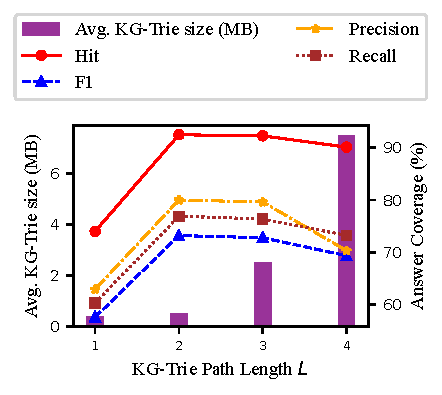
\includegraphics[width=.4\columnwidth]{images/l-hop.pdf}
    \end{center}
  %   \vspace{-14pt}
    \caption{Parameter analysis of path hop $L$ for KG-Trie construction on WebQSP.}
  %   \vspace{-16pt}
  \label{fig:l-hop}
\end{figure}

\RE{
    \subsection{Performance on Multi-path Reasoning}\label{app:multi_paths}

    GCR could take advantage of the GPU parallel computation to conduct multi-path explorations on KGs with beam-search. It could generate simultaneously generate $K$ reasoning paths and hypothesis answers with beam search in a single LLM call. The effectiveness of different $K$ is analyzed in \Cref{fig:beam-size} where larger $K$ can lead to a better recall of the answers. In addition, we compare the F1 performance under different numbers of ground-truth answers with RoG, which requires reasoning across multiple reasoning paths to find all answers. From the results shown in \Cref{tab:multi_path}, we can observe that GCR exhibits better performance in exploring multiple paths for reasoning.

    \begin{table}[h]
        \centering
        \caption{F1 comparison against RoG under different numbers of ground-truth answers.}
        \label{tab:multi_path}
        \resizebox{\textwidth}{!}{%
            \begin{tabular}{@{}c|cccc|cccc@{}}
                \toprule
                \multirow{2}{*}{Methods} & \multicolumn{4}{c|}{WebQSP} & \multicolumn{4}{c}{CWQ}                                                                                                                                                                                                           \\ \cmidrule(l){2-9}
                                         & \# Ans = 1                  & 2 \textless{}= \# Ans \textless{}= 4 & 5 \textless{}= \# Ans \textless{}= 9 & \# Ans \textgreater{}= 10 & \# Ans = 1    & 2 \textless{}= \# Ans \textless{}= 4 & 5 \textless{}= \# Ans \textless{}= 9 & \# Ans \textgreater{}= 10 \\ \midrule
                GCR                      & \textbf{71.31}              & 78.14                                & \textbf{83.47}                       & \textbf{63.20}            & 55.80         & \textbf{64.08}                       & \textbf{62.57}                       & \textbf{55.32}            \\
                RoG                      & 67.89                       & \textbf{79.39}                       & 75.04                                & 58.33                     & \textbf{56.9} & 53.73                                & 58.36                                & 43.62                     \\ \bottomrule
            \end{tabular}%
        }
    \end{table}

    \subsection{Performance on Multi-hop Reasoning}\label{app:multi_hops}
    To demonstrate the effectiveness of multi-hop reasonings. We illustrate the F1 performance under different hops. From results shown in \Cref{tab:multi_hops}, we can observe that GCR also outperforms baselines in multi-hop reasoning.

    \begin{table}[h!]
        \centering
        \caption{F1 comparison against RoG under different hops of reasoning.}
        \label{tab:multi_hops}
        % \resizebox{\textwidth}{!}{%
        \begin{tabular}{@{}c|cccccc@{}}
            \toprule
            \multirow{2}{*}{Methods} & \multicolumn{3}{c}{WebQSP} & \multicolumn{3}{c}{CWQ}                                                                                                      \\ \cmidrule(l){2-7}
                                     & 1 hop                      & 2 hop                   & \multicolumn{1}{c|}{\textgreater{}=3 hop} & 1 hop          & 2 hop          & \textgreater{}=3 hop \\ \midrule
            GCR                      & 75.05                      & \textbf{72.72}          & \multicolumn{1}{c|}{-}                    & \textbf{64.54} & \textbf{62.44} & \textbf{43.82}       \\
            RoG                      & \textbf{77.03}             & 64.86                   & \multicolumn{1}{c|}{-}                    & 62.88          & 58.46          & 37.82                \\ \bottomrule
        \end{tabular}%
        % }
    \end{table}
}

\subsection{Logical Coherence in KG Reasoning Paths}\label{app:logical_coherence}
Due to the lack of ground truth and a great number of paths, we utilize the LLMs to evaluate the logical coherence and semantic meanings of the generated paths. The prompt is shown in \Cref{fig:path_eval_prompt}. The LLMs are asked to evaluate the logical coherence of the generated paths and provide a score from 1 to 5. The results show that GCR achieves an average \textbf{3.9} in evaluation score, which demonstrates the logical coherence of the generated paths. Moreover, the LLM-based evaluation can be further used for selecting meaningful paths for training.

\begin{figure}[htb]
    \centering
    \begin{minipage}{0.99\columnwidth}
        \centering
        \begin{tcolorbox}[title=Path Evaluation Prompt]
            \small
            \begin{lstlisting}
============================= Prompt Input ================================
    
As an advanced reasoning evaluator, your task is to analyze whether the following reasoning path presents a **logically coherent connection from the question (subject entity) to the answer (target entity)**. You will assess whether each step in the path is valid and necessary, and whether the overall reasoning supports the final answer in a grounded and justified manner.

### Instructions:
1. Focus on whether the reasoning path makes logical sense from the question to the answer.
2. Check whether each relation contributes meaningfully and validly to reaching the final answer.
3. Penalize paths that make unjustified jumps, overly general connections, or weak associations.

### Rating Scale:
5 - Excellent: Every step is logically valid and contributes clearly toward the answer.  
4 - Good: Mostly coherent with minor assumptions or weak steps.  
3 - Moderate: Some steps are unclear, general, or weak, but the general direction is acceptable.  
2 - Poor: Contains major logical leaps or unclear connections.  
1 - Very Poor: Illogical or invalid path from question to answer.

### Output:
- Score: [1 to 5]  
- Explanation: [Brief explanation of the logical quality of the path from question to answer]

### Question:
<Question>
### Answer:
<Answer>
### Path:
<Path>
============================= LLM Output ================================
<Score>
            \end{lstlisting}
        \end{tcolorbox}
        \vspace{1mm}
    \end{minipage}
    \caption{The prompt template for path evaluation.}
    \label{fig:path_eval_prompt}
\end{figure}

\RE{
    \subsection{Analysis of the Failure Cases}\label{app:failure}
    Although GCR achieves 100\% trustful reasoning, there are still some failure cases due to the noise and redundant information in KGs. Two failure cases are presented in \Cref{tab:failures}. In the first case, the generated path is unrelated to the question. GCR provides a valid reasoning path that describes Anna Bligh's political position, which lacks information about her electoral district. Although LLMs exhibit strong reasoning ability, they still cannot always find meaningful paths, resulting in incorrect answers.
    %
    In the second case, the KG is incomplete, and the generated path does not contain facts for generating answers. Although KGs store abundant factual knowledge, there are still missing facts. Because there is no information about the character's player stored in KGs, GCR cannot generate the correct answer.
    These failure cases indicate that the performance of \ourmethod can be further improved by enhancing the reasoning ability of LLMs and the completeness of KGs.
    \begin{table}[h!]
        \centering
        \caption{Failure cases predicted by \ourmethod.}
        \label{tab:failures}
        \resizebox{.9\columnwidth}{!}{%
            \begin{tabular}{@{}c|p{5in}@{}}
                \toprule
                \multicolumn{2}{l}{\textbf{Case 1}: Generated paths are unrelated to the questions.}                                                                                                                                                               \\
                \midrule
                Question         & What electorate does anna bligh representt?                                                                                                                                                                                     \\ \midrule
                Answer           & Electoral district of South Brisbane                                                                                                                                                                                            \\ \midrule
                Generated Path   & \begin{tabular}[c]{@{}p{5in}@{}} Anna Bligh $\to$ government.politician.government\_positions\_held $\to$ m.0cr320w $\to$ government.government\_position\_held.jurisdiction\_of\_office $\to$ Queensland\end{tabular}          \\\midrule
                Predicted answer & \textcolor{red}{Queensland}                                                                                                                                                                                                     \\\midrule\midrule
                \multicolumn{2}{l}{\textbf{Case 2}: KG incompleteness.}                                                                                                                                                                                            \\
                \midrule
                Question         & who plays ken barlow in coronation street?
                \\ \midrule
                Answer           & William Roache                                                                                                                                                                                                                  \\ \midrule
                Generated Path   & \begin{tabular}[c]{@{}p{5in}@{}} Coronation Street $\to$ tv.tv\_program.program\_creator $\to$ Tony Warren $\to$ fictional\_universe.fictional\_character\_creator.fictional\_characters\_created $\to$ Ken Barlow\end{tabular} \\\midrule
                Predicted answer & \textcolor{red}{ Ken Barlow}                                                                                                                                                                                                    \\
                \bottomrule
            \end{tabular}}
    \end{table}


}

% \RE{
% \subsection{Performance  comparison with GNN-based graph reasoning methods}\label{app:gnn}

% Graph neural networks \citep{wu2020comprehensive} have shown impressive reasoning ability on KGQA tasks. In this section, we compare the performance of \ourmethod with GNN-based graph reasoning methods, e.g., GraftNet \citep{sun2018open}, UniKGQA \citep{jiang2022unikgqa}, and ReaRev \citep{mavromatis2022rearev}. The results are shown in \Cref{tab:gnn}. We observe that \ourmethod outperforms all the GNN-based graph reasoning methods on both WebQSP and CWQ datasets. This indicates that \ourmethod can effectively leverage the KG constraints to guide the LLMs to conduct faithful reasoning on KGs. The performance of \ourmethod is competitive with the state-of-the-art GNN-based graph reasoning methods. This demonstrates that \ourmethod can achieve comparable performance with GNN-based methods while maintaining the flexibility and efficiency of LLMs.

% \begin{table}[]
%     \centering
%     \caption{Comparison with GNN-based graph reasoning baselines.}
%     \label{tab:gnn}
%     % \resizebox{\textwidth}{!}{%
%     \begin{tabular}{@{}l|ll|ll@{}}
%     \toprule
%     \multirow{2}{*}{Methods}         & \multicolumn{2}{l|}{WebQSP} & \multicolumn{2}{l}{CWQ} \\ \cmidrule(l){2-5} 
%                                      & Hit          & F1           & Hit        & F1         \\ \midrule
%     GraftNet \citep{sun2018open}                 & 66.7         & 62.4         & 36.8       & 32.7       \\
%     UniKGQA \citep{jiang2022unikgqa}                  & 77.2         & 72.2         & 51.2       & 49.1       \\
%     ReaRev \citep{mavromatis2022rearev}                   & 76.4         & 70.9         & 52.9       & 47.8       \\ \midrule
%     GCR (Llama-3.1-8B + ChatGPT)     & 92.6         & 73.2         & 72.7       & 60.9       \\
%     GCR (Llama-3.1-8B + GPT-4o-mini) & 92.2         & 74.1         & 75.8       & 61.7       \\ \bottomrule
%     \end{tabular}%
%     % }
%     \end{table}

% }
% \subsection{Performance on Different Beam-sizes}\label{app:beam}
% We also analyze the impact of different beam sizes for graph-constrained decoding on the performance of \ourmethod. We conduct the experiments on WebQSP with different beam sizes of 1, 3, 5, 10, and 20. The results are shown in \Cref{fig:beam-size}. We observe that the hit and recall of \ourmethod increase with the beam size. Because, with a larger beam size, the LLMs can explore more reasoning paths and find the correct answers. However, the F1 score, peaks when the beam size is set to 10. This is because the beam size of 10 can provide a balance between the exploration and exploitation of the reasoning paths. When the beam size is set to 20, the performance drops due to the increased complexity of the search space, which may introduce noise and make the reasoning less reliable. Although the graph-constrained decoding benefits from the parallel GPU computation to explore multiple reasoning paths at the same time, the time cost still slightly increases from 1.4s to 7.8s with the increase of the beam size. Thus, we set the beam size to 10 for the following experiments to balance the performance and efficiency.

% % \begin{wrapfigure}{r}{0.55\columnwidth}
%   \vspace{-10pt}
\begin{figure}[]
    \begin{center}
        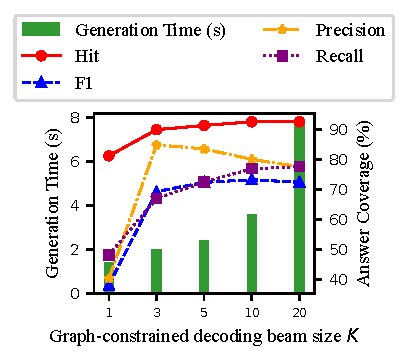
\includegraphics[width=.7\columnwidth]{images/k-beam.pdf}
      \end{center}
      \vspace{-20pt}
      \caption{Parameter analysis of beam size $K$.}
    \label{fig:beam-size}
    \vspace{-14pt}
\end{figure}
% \end{wrapfigure}

\RE{
\section{Limitations}\label{app:limits}
In this section, we discuss the limitations and future directions of the proposed method.

\begin{itemize}
    \item \textbf{Definition of Zero-hallucination.} This paper defines KG-constrained zero-hallucination as the generated reasoning paths are fully grounded in the KG. However, KGs often face issues of incompleteness and incorrect facts, leading to occasional false positives. Detecting such hallucinations without external evidence remains challenging, highlighting the potential of integrating cross-references from multiple knowledge sources—such as KGs, web data, and documents—to improve reasoning faithfulness.
    \item \textbf{Time Complexity of Complex Questions.} Highly complex questions usually require conduct reasoning with multiple steps. However, directly constructing a KG-Trie for a larger $L$ can be time-consuming. To address this, GCR can be integrated with existing planning-based methods to decompose complex questions into multiple shorter steps \citep{li2024framework}. By breaking down the reasoning process, we can construct a KG-Trie with a smaller $L$ for each subtask to conduct reasoning, thereby reducing computational overhead while maintaining inference quality. 
    \item \textbf{Irrelevant Reasoning Path.} As shown in \Cref{app:failure}, although LLMs exhibit strong reasoning ability, they still cannot always find meaningful paths, resulting in incorrect answers. It is worth to investigate how to further improve the reasoning ability of LLMs, especially under the settings of incomplete knowledge graphs.
\end{itemize}

}

\section{Templates and Prompts}\label{app:prompts}
In this section, we illustrate all the templates and prompts used in the experiments.
 
\noindent\textbf{Path Sentence Template.} The template for converting reasoning paths into natural language sentences is shown in \Cref{fig:path_template}, where the $e_*$ and $r_*$ denotes the entities and relations in a reasoning path $\vw_\vz=e_0\xrightarrow{r_1}e_1\xrightarrow{r_2}\ldots\xrightarrow{r_l}e_{l}$,
\begin{figure}[h]
    \centering
    \begin{minipage}{0.99\columnwidth}
        \centering
        \begin{tcolorbox}[title=Path Sentence Template]
            \small
            \texttt{<PATH>} $e_1$ $\to$ $r_1$ $\to$ $e_2$ $\to$ $\ldots$ $\to$ $r_l$ $\to$ $e_l$ \texttt{</PATH>}
        \end{tcolorbox}
        % \vspace{1mm}
    \end{minipage}
    \caption{The template for converting reasoning paths into formatted sentences.}
    \label{fig:path_template}
\end{figure}

\noindent\textbf{Graph-constrained Decoding Prompt.}
The prompt for graph-constrained decoding is shown in \Cref{fig:path_gen_prompt}, where the question and mentioned entities are provided to the LLMs to generate reasoning paths and hypothesis answers. In the fine-tuning datasets, the supervised LLM outputs are constructed from the ground-truth answers and reasoning paths extracted from the KGs.
\begin{figure}[htb]
    \centering
    \begin{minipage}{0.99\columnwidth}
        \centering
        \begin{tcolorbox}[title=Graph-constrained Decoding Prompt]
            \small
            ============================= Prompt Input ================================
    
            Reasoning path is a sequence of triples in the KG that connects the topic entities in the question to answer entities. Given a question, please generate some reasoning paths in the KG starting from the topic entities to answer the question.
    
            \vspace{10pt}

            \# Question: 
            
            \texttt{<Question>}

            \vspace{10pt}

            \# Topic entities:

            \texttt{<Question Entities>}
    
            \vspace{10pt}
            ============================= LLM Output ================================
    
            \# Reasoning Path: 
            
            \texttt{<PATH>} \texttt{<Reasoning Path>} \texttt{</PATH>}

            \vspace{10pt}
    
            \# Answer: 
            
            \texttt{<Hypothesis Answer>}
        \end{tcolorbox}
        \vspace{1mm}
    \end{minipage}
    \caption{The prompt template for graph-constrained decoding.}
    \label{fig:path_gen_prompt}
\end{figure}

The few-shot prompt template for graph-constrained decoding is shown in \Cref{fig:few_shotpath_gen_prompt}. We provide a few examples in the prompts to guide the LLMs to generate reasoning paths. Since the LLMs with few-shot prompt learning are not fine-tuned on the graph-constrained decoding task, we only apply the constraint to generate reasoning paths.

\noindent\textbf{Graph Inductive Reasoning Prompt.} The prompt for graph inductive reasoning is shown in \Cref{fig:reasoning_prompt}. We adopt the graph-constrained decoding to generate $K$ reasoning paths and hypothesis answers for each question. The reasoning paths and hypothesis answers are provided to the general LLMs to answer the questions without fine-tuning.

\noindent\textbf{Path Evaluation Prompt.} The prompt for evaluating the logical coherence of reasoning paths is shown in \Cref{fig:path_eval_prompt}. The LLMs are asked to evaluate the logical coherence of the generated paths and provide a score from 1 to 5.

\begin{figure}[h]
    \centering
    \begin{minipage}{0.99\columnwidth}
        \centering
        \begin{tcolorbox}[title=Graph Inductive Reasoning Prompt]
            \small
            ============================= Prompt Input ================================
    
            \# Reasoning Paths:

            \texttt{<Reasoning Path 1>}\texttt{<Hypothesis Answer 1>}

            $\ldots$

            \texttt{<Reasoning Path K>}\texttt{<Hypothesis Answer K>}
            
            \vspace{10pt}

            \# Question: 
            
            \texttt{<Question>}

            \vspace{10pt}

            Based on the reasoning paths, please answer the given question. Please keep the answer as simple as possible and only return answers. Please return each answer in a new line.
            
            \vspace{10pt}
            ============================= LLM Output ================================
    
            \texttt{<Answer 1>}

            \texttt{<Answer 2>}

            $\ldots$
            
            
        \end{tcolorbox}
        \vspace{1mm}
    \end{minipage}
    \caption{The prompt template for graph inductive reasoning.}
    \label{fig:reasoning_prompt}
\end{figure}

\begin{figure}[h]
    \centering
    \begin{minipage}{0.99\columnwidth}
        \centering
        \begin{tcolorbox}[title=Few-shot Graph-constrained Decoding Prompt]
            \small
            ============================= Prompt Input ================================
    
            Reasoning path is a sequence of triples in the KG that connects the topic entities in the question to answer entities. Given a question, please generate some reasoning paths in the KG starting from the topic entities to answer the question.
    
            \vspace{10pt}

            Example 1

            \vspace{10pt}

            \# Question: 
            
            \texttt{<Question>}

            \vspace{10pt}

            \# Topic entities:

            \texttt{<Question Entities>}

            \vspace{10pt}

            \# Reasoning Path: 
            
            \texttt{<Reasoning Path>}

            \vspace{10pt}

            Example 2

            \vspace{10pt}

            \# Question: 
            
            \texttt{<Question>}

            \vspace{10pt}

            \# Topic entities:

            \texttt{<Question Entities>}

            \vspace{10pt}
            
            \# Reasoning Path: 
            
            \texttt{<Reasoning Path>}

            \vspace{10pt}

            Example 3

            \vspace{10pt}

            \# Question: 
            
            \texttt{<Question>}

            \vspace{10pt}

            \# Topic entities:

            \texttt{<Question Entities>}

            \vspace{10pt}
            
            \# Reasoning Path: 
            
            \texttt{<Reasoning Path>}

            \vspace{10pt}

            Input

            \vspace{10pt}

            \# Question: 
            
            \texttt{<Question>}

            \vspace{10pt}

            \# Topic entities:

            \texttt{<Question Entities>}
    
            \vspace{10pt}
            ============================= LLM Output ================================
    
            \# Reasoning Path: 
            
            \texttt{<Reasoning Path>}
        \end{tcolorbox}
        \vspace{1mm}
    \end{minipage}
    \caption{The few-shot prompt template for graph-constrained decoding.}
    \label{fig:few_shotpath_gen_prompt}
\end{figure}